
\vspace{10mm}
\noindent
In the previous chapter,
  we laid out our need
  for tooling
  which can allow us
  to reason about tensor programs
  flexibly.
While developing the 3LA methodology~\cite{huang2024application},
  we needed a 
  tool 
  which would allow us to find opportunities
  to invoke accelerators
  within machine learning workloads.
TVM's Bring Your Own Codegen (BYOC)~\cite{chen2021byoc} framework
  was ostensibly designed for this purpose,
  but as we saw,
  BYOC was not flexible enough
  for the workloads we cared about.
  

To increase the likelihood of finding matches,
  pattern matching often relies on
  additional transformations
  to canonicalize intermediate representations (IRs)
  and massage data layouts into
  formats matching accelerator requirements~\cite{nvidia2020nhwc,newcomb2020halide-rewrite,
  hagedorn2020func-high-perf}.
Put in terms of our thesis,
  these transformations increase the
  \textit{flexibility}
  of our underlying matching \cref{thesis:algorithms},
  pushing us further up in our 
  algorithm adaptability--model explicitness spectrum
  (\cref{fig:intro:model-alg-spectrum}).
Once we start modifying the source program
  to find matches,
  the problem of mapping to accelerators
  becomes a \textit{term rewriting} problem,
  and thus
  we should be able to take advantage of
  the wealth of existing knowledge on 
  term rewriting techniques~\cite{baader1998term}.

Term rewriting is a well-known technique 
  for program transformations,
  with some compiler optimizations being implemented
  as term-rewriting systems~\cite{
    dershowitz1993taste,
    baader1999term,
    blindell2016instruction,
    regis-pact22}.
%to transform program fragments to equivalent program fragments. 
Given a set of syntactic rewrite rules ($\ell \rightarrow r$) that also preserve semantic equality, 
  a term-rewriting system 
  rewrites instances of pattern $\ell$ 
  in the input program with semantically equivalent pattern $r$ where applicable.
%If all the rules preserve semantic equality,
%  then the application of multiple rules
%  also preserves equality,
%  allowing for modular correctness checking 
%  by verifying the individual rewrite rules.
%It has a variety of applications in compilers including replacing a program with an equivalent program that is optimal for some cost function. 

One term rewriting approach
  of particular interest
  is \gls{equality-saturation}.
In traditional term rewriting,
  % the ordering of rewrites is important,since 
  applying one rewrite rule
  may prevent
  using other, potentially profitable, rewrite rules;
  this is referred to as the phase-ordering problem~\cite{whitfield1997approach}.
  %and it may impact the quality of the final results
Equality saturation avoids
  phase-ordering issues % when applying rewrites
  by searching over many equivalent rewritings of the same program~\cite{tate2011equality,joshi2002denali}.
  %including different choices of accelerator operations, which ultimately 
  %reduces the need for manual program restructuring.
%  and improves application portability.
Given an input program $p$, 
  equality saturation repeatedly applies 
  the given rewrite rules 
  to explore all equivalent ways to express $p$
%  (with respect to the rewrite rules and resource limits)
%This is accomplished 
using an \textit{e-graph} data structure
  to efficiently represent an exponentially large set of equivalent program expressions~\cite{nelson1980fast,nieuwenhuis2005proof}.
Upon reaching a fixed point, 
  i.e., when no application of any rewrite rule can introduce a new program expression,
  or upon hitting a predetermined resource limit,
  the optimal rewritten program
  can be extracted from an e-graph
  according to a given cost function.
  % thus providing for searching over many candidate rewritings 
  % without sophisticated ordering considerations. 

To increase flexibility
  of accelerator mapping \cref{thesis:algorithms},
  {\TLA} sought to employ equality saturation;
  unfortunately, existing IRs in compilers for
  array/tensor programming DSLs 
  are not compatible with equality saturation.
Equality saturation is most easily applied in
  \textit{pure} (side effect--free) IRs
  that support equational reasoning.
Due to their purity, these IRs tend to be
  high-level.
However,
  mapping to accelerators requires considering
  low-level hardware details like data layout.
Existing pure IRs for ML frameworks are used
  primarily for high-level transformations
  (e.g., type elaboration and inlining)
  and do not expose low-level data layout details~\cite{relay}.
On the other hand,
  IRs used for crucial lower-level optimizations like
  operator fusion must support
  precise reasoning about memory use,
  and therefore are typically impure,
  hampering term rewriting.
In summary, for our purposes,
  existing IRs are either pure but too high-level,
  or low-level enough but impure.

To help mitigate such impedance mismatches,
  we present \textit{\g},\footnote{Publicly available at \url{https://github.com/gussmith23/glenside}.}
  a pure tensor program IR
  that enables hardware-level term rewriting.
\g is based on a simple
  \textit{access pattern} abstraction that
  supports expressing and reasoning about
  data layout transformations via
  syntactic rewrite rules.
% We moved this figure elsewhere in the thesis
%   \begin{wrapfigure}{r}{.5\textwidth}
%     \centering
%     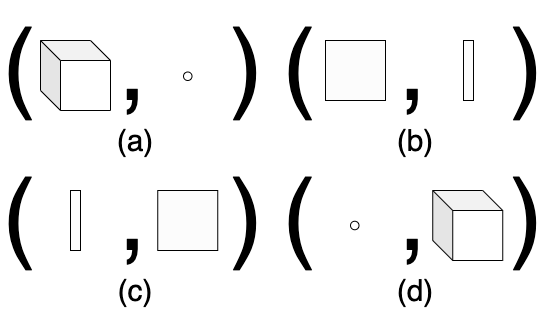
\includegraphics[width=.9\linewidth]{glenside/access-pattern-examples-2x2.png}
%     \caption{
%       Four access patterns,
%         representing different ways
%         a
%         tensor program
%         (or \textit{kernel})
%         might access
%         the same 3D tensor. 
%       For example, (c) represents
%         accessing a 3D tensor as
%         a vector of 2D matrices.}
%     \label{fig:access-pattern-examples}
%     \vspace{-1em}
% \end{wrapfigure}
When combined with standard arithmetic rewrites
  for per-tensor-element computations,
  access patterns enable implementing complex
  transformations for accelerator support as
  compositions of simple rewrites.

\begin{figure}
    \centering
    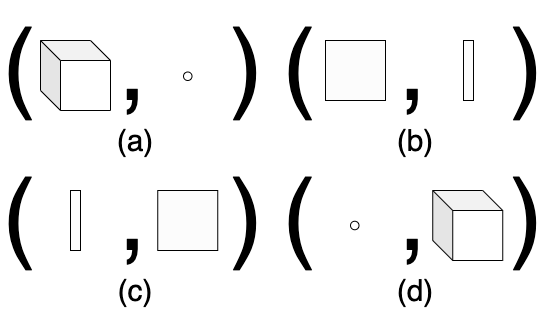
\includegraphics[width=.6\linewidth]{glenside/access-pattern-examples-2x2.png}
    \caption{
      Four access patterns,
        representing different ways
        a
        tensor program
        (or \textit{kernel})
        might access
        the same 3D tensor. 
      For example, (c) represents
        accessing a 3D tensor as
        a vector of 2D matrices.}
    \label{fig:access-pattern-examples}
    \vspace{-1em}
\end{figure}

Tensors are traditionally characterized
  by their \textit{shape},
  an $n$-tuple 
  %in $\mathbb{N}^n$
  of positive integers
  indicating the size of each
  of a tensor's dimensions.
  % , e.g., $(x, y, z)$ for a 3D tensor.
Access patterns instead characterize
  each tensor with two shapes, e.g.,
  \accesspatternshape{x}{y, z}, separating
  the dimensions which are \textit{iterated over} from
  the dimensions which are \textit{computed on.}
Figure~\ref{fig:access-pattern-examples}(c)
  depicts an example where a 3D tensor's
  first dimension is iterated over and
  some computation applied to each
  corresponding 2D matrix.

% \hl{todo: this should probably moved up?}
% We demonstrate how \g
%   enables implementing representative
%   hardware-level transformation via term rewriting,
%   including mapping computations
%   to systolic arrays~\cite{jouppi2017tpu}
%   (a common hardware module in ML accelerators)
%   and automatically discovering the
%   \tcd{im2col} data layout transformation~\cite{im2col},
%   which enables mapping 2D convolutions
%   to matrix multiplication hardware.
% In particular,
%   by employing \textit{equality saturation}~\cite{willsey2021egg},
%   these transformations ``fall out for free''
%   (i.e., without any carefully crafted
%   rewrite orderings~\cite{phase-ordering}),
%   from a handful of general rewrites concerning tensor
%   transposition, Cartesian product, dot product, etc.,
%   expressed in terms of access patterns.
% \hl{end todo}

In the rest of this chapter,
  we will first walk through an example
  demonstrating the difficulty
  in developing a pure tensor IR
  \cref{sec:matmul}.
We will then describe  
  the implementation of \g in
  \cref{sec:glenside}.
Lastly, we describe how \g
  was incorporated into \TLA
  in \cref{sec:glenside-in-3la}.
